\documentclass[11pt]{article}
\usepackage{amsmath}
%\usepackage{extsizes}
\usepackage{amsmath,amssymb}
%\usepackage{omegavn,ocmrvn}
%\usepackage[utf8x]{inputenc}
\usepackage[utf8]{vietnam}

\usepackage{longtable}
\usepackage{answers}
\usepackage{graphicx}
\usepackage{array}
\usepackage{pifont}
\usepackage{picinpar}
\usepackage{enumerate}
\usepackage[top=3.0cm, bottom=3.5cm, left=3.5cm, right=2.5cm] {geometry}
\usepackage{hyperref}


\newtheorem{bt}{Câu}
\newcommand{\RR}{\mathbb R}
\Newassociation{sol}{Solution}{ans}
\newtheorem{ex}{Câu}
\renewcommand{\solutionstyle}[1]{\textbf{ #1}.}
\newcommand{\m}[1]{
	\begin{bmatrix}
		#1 
	\end{bmatrix}
}


\begin{document}
% \noindent
\begin{tabular*}
{\linewidth}{c>{\centering\hspace{0pt}} p{.7\textwidth}}
Trường ĐHKHTN, ĐHQGHN & {\bf Học Kỳ 2 (2020-2021)}
\tabularnewline
K63 TTƯD & {\bf Bài tập giữa kỳ}
\tabularnewline
\rule{1in}{1pt}  \small  & \rule{2in}{1pt} %(Due date:)
\tabularnewline

%  \tabularnewline
%  &(Đề thi có 1 trang)
\end{tabular*}
%
% \Opensolutionfile{ans}[ans1]

\begin{bt}
Hãy dịch và đánh máy lại ví dụ được phân công, LATEX hay Word tùy các em chọn.
\end{bt}

\begin{bt}
Sử dụng mô hình được phân công, hãy lập trình để thực hiện các nhiệm vụ sau. \\
i) Tìm hàm truyền của hệ, tìm các cực, không điểm của hệ. \\
ii) Vẽ đồ thị phản hồi đầu vào 0 (với trạng thái ban đầu $x_0$ là vector gồm toàn số $1$) \\ 
iii) Sử dụng hàm đầu vào $u$ là hàm xung (xem lệnh impulse trong MATLAB) và hàm bước nhảy (xem lệnh step trong MATLAB) hãy vẽ riêng đồ thị của $u$
và đồ thị của hàm phản hồi trạng thái 0 (với 2 hàm đầu vào trên) \\
\end{bt}

\begin{bt}
Hãy tìm phép đổi biến số thích hợp để chia tỉ lệ (magnitude scaling) hệ sau, sao cho tất cả các biến trạng thái $x_i(t)$ đều có độ lớn bằng với độ lớn tối đa của đầu ra $y(t)$. 
%
\begin{align*}
&\dot{x} = \m{-2 & 0 & 0\\1 & 0 & 1 \\ 0 & -2 & -2} x + \m{1 \\ 0 \\ 1} u, \\
& y = \m{1 & -1 & 0} x
\end{align*}
%
Nếu mọi tín hiệu đều phải nằm trong phạm vi $\pm10$ V và nếu hàm đầu vào là hàm bước nhảy (step với độ lớn $a$) thì $a$ tối đa có thể là bao nhiêu? 	
\end{bt}

\begin{bt} BT để ôn lại về 2 hệ tương đương (equivalent) và tương đương trạng thái 0 (zero-equivalent) . \\
Hai hệ sau có tương đương hay không? Có tương đương zero hay không?
\begin{figure}[h!]
	\centering
	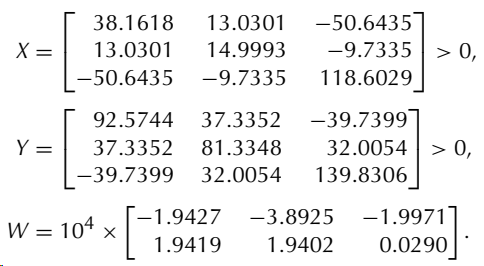
\includegraphics[width=0.7\linewidth]{screenshot001}
	%\caption{}
	\label{fig:screenshot001}
\end{figure}
\end{bt}

\centerline{———————————Hết——————————-}

\end{document}


